\chapter{Przegląd badań}
\label{chapter:przegladbadan}
\begin{comment}
- dużo literatury, przegląd wiedzy dostępnej na dany temat
- sieci społeczne: SNA + analiza zachowań + grupy
- analiza sentymentu: techniki, itd
- twitter
- badania nad geolokacją, zastosowanie, jak
\end{comment}

W niniejszym rozdziale znajduje się aktualny stan badań dotyczący 4 tematów,
które składają się na tę pracę. Na początku opisana jest dziedzina sieci
społecznych, czym ta nauka się zajmuje, w jakich przypadkach może zostać
zastosowana.
Następnie omówiona zostaje analiza sentymentu wypowiedzi i przetwarzanie tekstu
celem ekstrakcji jego wydźwięku.
Później skupiam się nad temat związanym z geolokacją i opisem, co można dzięki
niej się dowiedzieć, a rozdział kończę omówieniem serwisu społecznościowego Twitter,
który został wykorzystany jako źródło danych do analizy sieci społecznych.








% %%%%%%%%%%%%%%%%%%%%%%%%%%%%%%%%%%%%%%%%%%%%%%%%%%%%%%%%%%%%%%% SIECI
% SPOŁECZNE
\section{Sieci społeczne}
Termin ten został użyty po raz pierwszy w 1954 roku przez Johna Arundela Barnesa
\cite{JABarnes}. Oznacza strukturę społeczną, którą tworzą jednostki (np. osoby
lub organizacje) i połączenia między nimi.
Analiza sieci społecznych jest badaną od wielu lat dziedziną nauki. Szybki
rozwój Internetu w XXI wieku wzbogacił ją o bogate źródło danych. Główne obszary
badań \cite{SNDAtopics} to między innymi:
\begin{itemize}
  \item statystyczna analiza sieci społecznych -- opisuje jak wygląda typowa sieć społeczna,
  badane są połączenia między jednostkami, aby sprawdzić czy posiadają kilka połączeń,
  czy sieć zbudowana jest z hubów (osobniki mające dużą liczbę połączeń, 
  łączące ze sobą różne części sieci społecznej; wokół nich koncentrują się inne
  jednostki), czy może liczba połączeń rozłożona jest równomiernie,
  
  \item odkrywanie grup/społeczności -- jest jednym z głównych tematów analizy 
  sieci społecznych; szukanie grup związane jest z klastrowaniem i odkrywaniem 
  obszarów sieci, które są bardziej zagęszczone (czyli takie, w których
  stosunek liczby krawędzi do liczby wierzchołków jest większy niż na zewnątrz);
  problem powiązany jest z badaniem grafów, określaniem jak dzielić sieć na regiony,
  
  \item klasyfikacja wierzchołków -- polega na opracowaniu metody, dzięki której
  możliwe jest zaklasyfikowanie wierzchołków do wcześniej zdefiniowanych klas na
  podstawie podobieństwa z innymi jednostkami do tych klas już należących,
  
  \item odnajdywanie ekspertów -- sieci społeczne mogą być używane jako narzędzia
  w celu odkrywania ekspertów do danego zadania,
  
  \item predykcja przyszłych połączeń wewnątrz sieci -- wiele badań skupia
  się na statycznych połączeniach wierzchołków; w wielu sieciach jednak 
  połączenia między węzłami są dynamiczne i badania te koncentrują się na 
  tym by przewidzieć nowe połączenia wewnątrz sieci,
  
  \item ekstrakcja wiedzy z sieci -- polega na eksploracji danych z mediów 
  społecznościowych i eksploracji tekstu z serwisów społecznościowych; 
  eksploracja danych dostarcza naukowcom narzędzia do analizy dużych, 
  złożonych i często zmieniających się danych wewnątrz sieci, a eksploracja tekstu
  może prowadzić do odkrycia nowych połączeń między węzłami i nowych
  charakterystyk je łączących; jej użycie wpływa na poprawę jakości
  badanej sieci. 
\end{itemize}



\subsection{Przykłady zastosowania analizy sieci społecznych}
Wyniki badań nad sieciami społecznymi stwarzają wiele możliwości dla różnych
dziedzin życia. Mogą być zastosowane między innymi przez:
\begin{itemize}
  \item służby porządkowe -- policja może przy ich pomocy odkrywać powiązania
  między przestępcami i dochodzić do zależności między grupami przestępczymi,
  a także odkrywać, kogo dane grupy mogłyby zwerbować; odkrywać siatki 
  przestępcze \cite{SNACriminal},
  
  \item badania naukowe -- odkrywanie naukowców zajmujących się podobnymi
  tematami celem opracowania bardziej kompletnych wyników lub podjęcia nowego,
  wspólnego tematu \cite{SNAScientists},
  
  \item przedsiębiorstwa handlowe -- odkrywanie zbliżonych typów klientów i 
  oferowanie im produktów lub usług do nabycia przy użyciu systemów 
  rekomendujących \cite{SNAReccomendation},
  
  \item służby zdrowotne -- użycie sieci społecznych może pomóc w określaniu
  obszarów, w które rozprzestrzeniają się wirusy groźnych chorób, dzięki czemu
  możliwe może być zapobieganie ich dalszej ekspansji \cite{SNAEpidemic}.
  
    
\end{itemize}



\subsection{Reprezentacja sieci społecznych}
Najczęściej spotykaną reprezentacją sieci społecznych jest reprezentacja
grafowa. Grafem nazywamy strukturę G = (V, E) składającą się z węzłów
(wierzchołków, oznaczonych przez V) wzajemnie połączonych za pomocą krawędzi
(oznaczanych przez E). Przykładowy graf został zaprezentowany na rysunku
\ref{image:graf-zwykly}.

\begin{figure}[ht!]
\centering
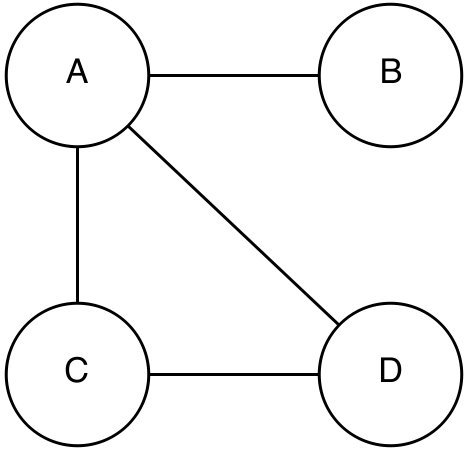
\includegraphics[width=40mm]{img/graf-zwykly.png}
\caption{Graf o 4 wierzchołkach i 4 krawędziach}
\label{image:graf-zwykly}
\end{figure}

Reprezentacja grafowa w naturalny sposób modeluje jednostki jako węzły i relacje
między nimi jako krawędzie. W zależności od rodzaju sieci graf taki może
posiadać krawędzie skierowane lub nieskierowane oraz ważone lub nieważone.
Krawędź skierowana reprezentuje kierunek, w którym przebiega komunikacja między
węzłami. Krawędź ważona może reprezentować  liczbę wiadomości wymienionych
między węzłami lub jakiś inny rodzaj wagi (oznaczania jednych krawędzi
za bardziej istotne od innych). Przykładowy graf skierowany o krawędziach ważonych
przedstawia rysunek \ref{image:graf-skierowany}.

\begin{figure}[ht!]
\centering
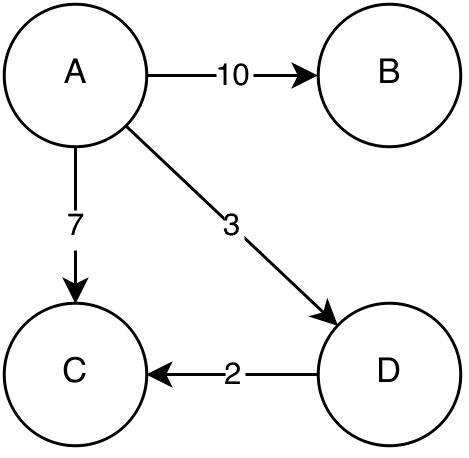
\includegraphics[width=40mm]{img/graf-skierowany.png}
\caption{Graf skierowany o krawędziach ważonych}
\label{image:graf-skierowany}
\end{figure}
















%%%%%%%%%%%%%%%%%%%%%%%%%%%%%%%%%%%%%%%%%%%%%%%%%%%%%% MIARY I POJĘCIA GRAFOWE

\subsection{Miary i pojęcia grafowe}
Zamodelowanie sieci społecznych w postaci grafów pozwala na skorzystanie z szeregu
miar związanych z tą dziedziną wiedzy. Dzięki nim możliwe jest odnajdywanie cech
charakterystycznych danej sieci. Najważniejsze miary pomagające odnaleźć najważniejsze
węzły to \cite{estrada}: 


\subsubsection{Stopień wierzchołka}
Miara określająca liczbę krawędzi wchodzących i 
  wychodzących z wierzchołka (patrz rys. \ref{image:stopien-wierzcholka})
  
\begin{figure}[ht!]
\centering
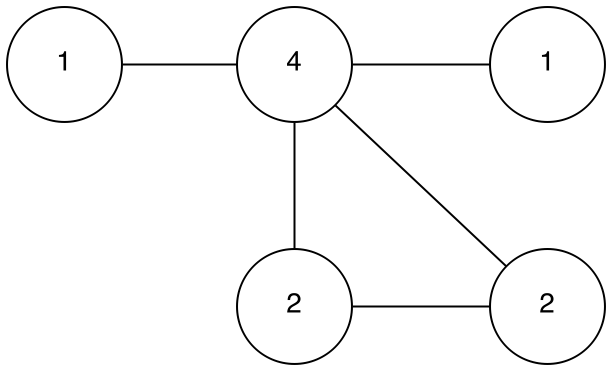
\includegraphics[width=80mm]{img/stopien-wierzcholka.png}
\caption{Graf z oznaczonymi stopniami wierzchołków}
\label{image:stopien-wierzcholka}
\end{figure}

W przypadku grafów skierowanych możemy jeszcze mówić o stopniu wchodzącym 
(ang. \textit{in degree}) oraz wychodzącym (ang. \textit{out degree}) 
(patrz rys. \ref{image:stopien-wierzcholka-skierowany}).
  
\clearpage
\begin{figure}[ht!]
\centering
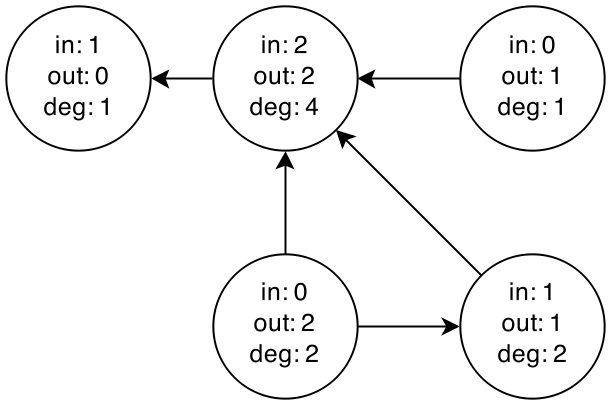
\includegraphics[width=80mm]{img/stopien-wierzcholka-skierowany.png}
\caption{Graf skierowany z oznaczonymi stopniami wierzchołków}
\label{image:stopien-wierzcholka-skierowany}
\end{figure}
  
  
\subsubsection{Pośrednictwo (ang. \textit{betweenness}) }  
Liczba najkrótszych ścieżek w grafie, które przechodzą przez dany węzeł podzielona
przez liczbę wszystkich najkrótszych ścieżek grafu. Przez najkrótszą ścieżkę 
rozumie się taką ścieżkę między dwoma węzłami grafu, dla której liczba krawędzi
jest najmniejsza.
  
\begin{equation}
BC(k) = \sum\limits_{i}\sum\limits_{j}\frac{\rho(i, k, j)}{\rho(i, j)}, \quad i \neq j \neq k
\end{equation}

gdzie:

$\rho(i, k, j)$ -- liczba najkrótszych ścieżek pomiędzy $i$ oraz $j$ przechodząca
przez wierzchołek $k$,

$\rho(i, j)$ -- liczba wszystkich najkrótszych ścieżek pomiędzy $i$ oraz $j$.

\bigskip

Przykładowo aby obliczyć wartość tej miary dla wierzchołka $B$ posłużmy się rysunkiem 
\ref{image:betweenness}.
Najkrótsze ścieżki między węzłami innymi niż $B$ to: $ABC,$ $ABD$, $ABE$, $CBD$, $CBE$, $DE$.
\mbox{W 5 z 6 z nich} znajduje się węzeł $B$, stąd wynika jego wartość \textit{betweenness}
równa $5/6$. 

\begin{figure}[ht!]
\centering
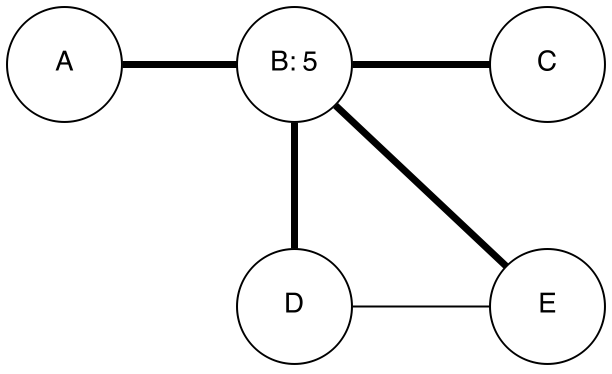
\includegraphics[width=80mm]{img/betweenness.png}
\caption{Najkrótsze scieżki przechodzące przez węzeł $B$}
\label{image:betweenness}
\end{figure}

Węzły o wysokiej wartości współczynnika \textit{betweenness} są interesujące
ponieważ mogą kontrolować przepływać informacji wewnątrz sieci oraz
mogą być zmuszone do przetwarzania większej ilości informacji.
Z tego wynika też, że mogą być skutecznym celem ataków.
    
  
\clearpage  
\subsubsection{Bliskość (ang. \textit{closeness})}  
Znormalizowana odwrotność sumy odległości między węzłami w grafie.
  
\begin{equation}
CC(k) = \frac{\sum\limits_{j}d(k, j)}{N - 1}
\end{equation}  

gdzie:

$d(k, j)$ -- odległość między wierzchołkami $k$ oraz $j$,

$N$ -- liczba wszystkich wierzchołków.

\bigskip

Wartość \textit{closeness} dla pojedynczego wierzchołka liczymy sumując
odległości między nim a pozostałymi wierzchołkami,
a następnie dzielimy tę wartość przez $N - 1$. Przykładowy graf \ref{image:closeness} i tabela 
\ref{tab:closeness} z obliczeniami tej wielkości znajdują się poniżej.


\begin{figure}[ht!]
\centering
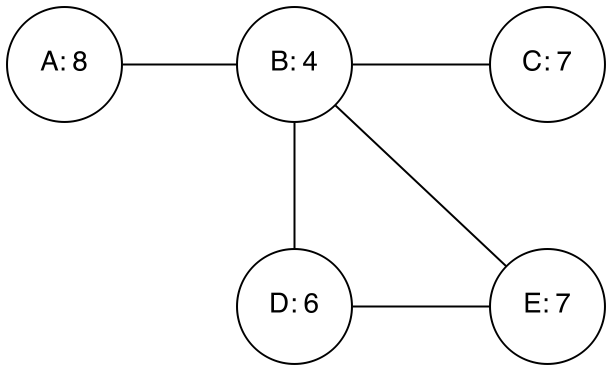
\includegraphics[width=80mm]{img/closeness.png}
\caption{Suma odległości do pozostałych węzłów w grafie}
\label{image:closeness}
\end{figure}
  

\begin{table}[ht!]  
\begin{center}  
\begin{tabular}{| c | c c c c c || c | c |}
 \hline
 & \multicolumn{5}{c ||}{Wierzchołki} & Suma odległości & Bliskość (\textit{closeness}) \\
 \hline
 & A & B & C & D & E &  $S = \sum\limits_{j}d(i, j)$ & $CC(i) = \frac{S}{N - 1} = \frac{S}{4}$ \\
\hline
A & 0 & 1 & 2 & 2 & 3 & 8 & 0.5 \\ 
B & 1 & 0 & 1 & 1 & 1 & 4 & \textbf{1.0} \\ 
C & 2 & 1 & 0 & 2 & 2 & 7 & 0.57 \\ 
D & 2 & 1 & 2 & 0 & 1 & 6 & 0.67 \\ 
E & 3 & 1 & 2 & 1 & 0 & 7 & 0.57 \\ 
 \hline
\end{tabular} 
\end{center} 
\caption{Odległości między węzłami i wartości miary \textit{closeness}}
\label{tab:closeness}
\end{table}
  
Węzłem o najmniejszej sumie odległości do innych wierzchołków -- a co za tym idzie --
o największej wartości bliskości jest węzeł $B$. Wynika z tego, że jest to
wierzchołek najszybciej rozsyłający informacje wewnątrz sieci pomiędzy jej elementami. 


\clearpage
\subsubsection{Wektor własny (ang. \textit{eigenvector})}
Miara centralności węzła,  która oceniając dany węzeł bierze także pod uwagę 
wartości jego sąsiadów (bezpośrednio przyległych węzłów).
Zastosowanie tej wielkości pozwala wskazać najważniejszy węzeł w sytuacji,
gdy poprzednie miary zwracają równe wyniki. Wartość tej wielkości wyraża się
wzorem:

\begin{equation}
EV(k) = \frac{1}{\lambda}\sum\limits_{j}A_{kj}x_j
\end{equation}

gdzie:

$\lambda$ -- stała, równa największej wartości własnej macierzy sąsiedztwa grafu,

\begin{math}
 A_{kj} =
  \begin{cases}
   1, \text{gdy wierzchołki $k$ oraz $j$ mają wspólną krawędź} \\
   0, \text{w przeciwnym wypadku}
  \end{cases}

\end{math}


\bigskip

Przykładowe wartości wielkości \textit{eigenvector}
zaprezentowano na rysunku \ref{image:eigenvector}. Wartości te zostały
obliczone przy pomocy narzędzia Gephi\footnote{https://gephi.github.io/}.

\begin{figure}[ht!]
\centering
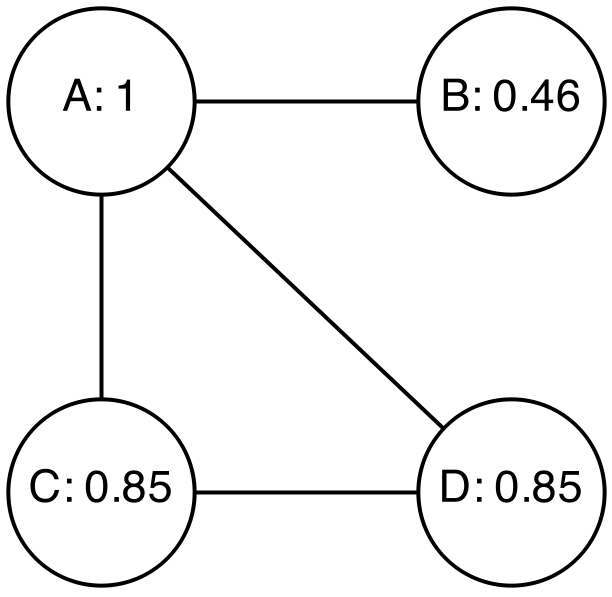
\includegraphics[width=40mm]{img/eigenvector.png}
\caption{Wartości wielkości \textit{eigenvector} w przykładowym grafie}
\label{image:eigenvector}
\end{figure}


\subsubsection{Klika}
W analizie sieci społecznych (traktowanych jako graf) przydatne są także 
2 następujące pojęcia:
\begin{itemize}
  \item klika -- podgraf grafu, w którym wszystkie wierzchołki połączone są 
  krawędzią,
  \item k-klika -- klika składająca się z dokładnie $k$-wierzchołków. Na przykład
  k-klika o $k=3$ to podgraf zbudowany z 3 wierzchołków, gdzie między każdym z 
  nich znajduje się krawędź (patrz rys. \ref{image:klika}).
\end{itemize}

\clearpage
\begin{figure}[ht!]
\centering
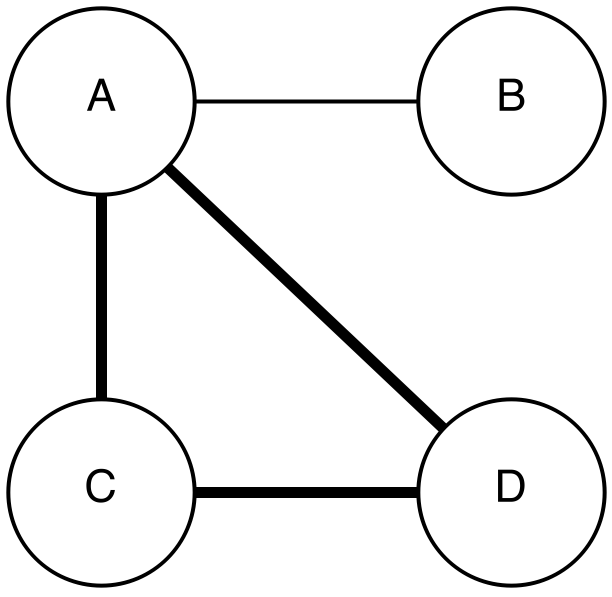
\includegraphics[width=40mm]{img/klika.png}
\caption{K-klika o rozmiarze 3 zbudowana przez wierzchołki $ACD$}
\label{image:klika}
\end{figure}








% %%%%%%%%%%%%%%%%%%%%%%%%%%%%%%%%%%%%%%%%%%%%%%%%%%%%%%%%%%%%%%%%%%%% SENTYMENT
\section{Sentyment wypowiedzi}
Sentyment (inaczej wydźwięk wypowiedzi) to stosunek lub postawa wobec jakiejś
sytuacji, zdarzenia. Badanie sentymentu niesie ze sobą bardzo dużo informacji.
Recenzje, komentarze i opinie odgrywają istotną rolę w ocenie satysfakcji z
produktu lub usługi czy w badaniu reakcji na wydarzenia. Dane, które zawierają
takie informacje mają bardzo wysoki potencjał w odkrywaniu wiedzy.
Dowiadywanie się, co myślą inni ludzie zawsze było bardzo istotne w procesie
podejmowania decyzji. Internet daje możliwość zapoznania się z opiniami innych
ludzi czy ekspertów. Możliwość analizy sentymentu wypowiedzi może być bardzo
pomocna. Jak wynika z badań przeprowadzonych na ponad 2000 dorosłych Amerykanów
\cite{pangLee} 81\% użytkowników Internetu przynajmniej raz poszukiwało w
Internecie informacji o jakimś produkcie z czego od 73\% do 87\% osób twierdzi,
że recenzje innych miały wpływ na ich wybory.

Zastosowanie analizy sentymentu jest bardzo szerokie. Niektóre
z obszarów jej użycia to \cite{pangLeeApplication}:
\begin{itemize}
  \item portale internetowe z opiniami -- zastosowanie analizy sentymentu
może być użyte do poprawy błędów popełnionych przez użytkowników (gdy opinia
jest pozytywna, a użytkownik omyłkowo wybrał niską ocenę) lub gdy opinie
są ewidentnie stronnicze, mogą pomóc w faktycznej ocenie danego przedmiotu czy 
usługi

\item jako technologia wspomagająca większe systemy -- analiza sentymentu może
być wsparciem dla systemów rekomendacji; na przykład może służyć do 
tego by nie rekomendować produktów, które otrzymały negatywne opinie; 
w systemach serwujących reklamy kontekstowe, wykrycie pozytywnego sentymentu
na stronie może być powodem wyświetlenia jakiejś reklamy,
a wykrycie negatywnego sentymentu powodem jej ukrycia;
innym zastosowaniem jest ekstrakcja informacji, która może być
polepszona poprzez pomijanie zdań subiektywnych, zawierających sentyment

\item biznes -- poprzez dostarczenie informacji o odbiorze sprzedawanych produktów
i serwowanych usług; gdy na przykład sprzedawany laptop ma negatywny odbiór
stosując analizę sentymentu można to bardzo szybko wykryć i dowiedzieć się
dlaczego zaistniała dana sytuacja; firma może badać swój ogólny odbiór
w społeczeństwie -- szybko reagować na niezadowolenie klientów, lub wprowadzać
poprawki do swoich produktów; wykrywanie sentymentu może również pomóc
przewidzieć wyniki sprzedaży

\item polityka -- użycie analizy sentymentu jest wręcz naturalne dla tego obszaru
życia; partie czy politycy mogą badać odbiór społeczeństwa swoich programów
i decyzji; badanie sentymentu może im na przykład wskazać w jakich miejscach,
czy przy jakich postaciach się pokazać by zyskać sympatię wyborców; istotne
również mogą być informacje na temat reakcji społeczeństwa na planowane
przez rząd zmiany w prawie. 
\end{itemize}

Krótko mówiąc największym zyskiem związanym z badaniem sentymentu jest możliwość
zbadania opinii bardzo dużej liczby osób w sposób mechaniczny. Nie ma potrzeby
przeprowadzania ankiet, pytania ludzi co sądzą na dany temat. Internauci samodzielnie
przedstawiają swoje opinie w Internecie, a przy pomocy analizy sentymentu bardzo
łatwe staje się zbadanie nastrojów.



Badanie sentymentu nie jest trywialne. Związane jest bezpośrednio z 
przetwarzaniem języka naturalnego, które niesie ze sobą szereg problemów
\cite{ChallengeOfSpokenLanguage}, \cite{NaturalLanguageProcessingFuture}:

\begin{itemize}
  \item złożoność języka naturalnego -- bardzo trudnym zadaniem jest nauczenie 
  programu komputerowego pełnego rozumienia języka naturalnego; co więcej każdy
  język jest inny, więc dla każdego konieczne jest zastosowanie różnych
  rozwiązań -- inaczej trzeba podejść do badania sentymentu w języku polskim
  a inaczej w angielskim; trzeba pamiętać też, że język naturalny nie jest
  martwy i ciągle się rozwija,

  \item trudność w analizie kontekstu wypowiedzi -- wykrycie ironii nie jest
  zadaniem prostym; bardzo często wypowiedzi mogą mieć związek z jakimś pojęciem
  zupełnie niezrozumiałym dla programu komputerowego, a oczywistym dla człowieka
  (np. idiomy, odniesienia do wydarzeń na świecie),

  \item slang w Internecie, skrótowce, literówki -- wszystkie te elementy
  dodatkowo utrudniają analizę sentymentu; użytkownicy Internetu nie zawsze
  dbają o jakość swojego języka, często stosują skróty, czy wyrażenia slangowe,
  które mogą być niezrozumiałe dla automatycznego analizatora sentymentu,

  \item SPAM, szum -- wszystkie wpisy, które nie niosą ze sobą żadnej wartości
  a pojawiają się w internetowych forach, serwisach z opiniami również stanowią
  wyzwanie przy budowie narzędzia do analizy sentymentu.

\end{itemize}





\subsection{Zastosowanie sentymentu w mediach społecznościowych}
Analiza sentymentu ma szerokie zastosowanie w analizie mediów społecznościowych.
Możliwość oceny wydźwięku wypowiedzi zamieszczanych przez internautów w sieci
prowadzi do interesujących wyników i na jej podstawie wyciągać można pomocne
wnioski. Na jej podstawie przeprowadzono wiele badań. 

W \cite{AgileSentimentAnalysis}
poprzez crawlowanie (z ang. przeszukiwanie stron i selekcjonowanie z nich
informacji) blogów związanych z Egiptem w 2011 roku badano nastroje
społeczeństwa w trakcie masowych demonstracji w tym kraju w związku z
niezadowoleniem rządzącymi. Sentyment pokazywał, że jeszcze przed rozpoczęciem
się demonstracji nastroje były bardzo negatywne. 

W \cite{SentimentRevealedInSocialMedia} porównany jest wpływ na giełdę artykułów
w \textit{Wall Street Jorunal} (nowojorska gazeta o tematyce gospodarczej) z
wpisami na \textit{Seeking Alpha} (popularny serwis społecznościowy skierowany
do osób grających na giełdzie). Artykuł udowadnia, że wpisy w \textit{Seeking
Alpha} mają większy i bardziej trwały wpis na zwracanie akcji niż opinie
wyrażane w \textit{Wall Street Journal}.

Z kolei w \cite{PresidentialElectionsOnTwitter} zostały przeprowadzone badania
nad sentymentem wpisów na Twitterze w kontekście wyborów prezydenckich we
Francji i Stanach Zjednoczonych.
Artykuł pokazuje, że sympatia do kandydatów wyrażana w internecie była wprost
propocjonalna do ich wyników sondażowych. W badaniach nad wyborami Francuskimi
więcej uwagi skupiał na sobie przegrany Nicolas Sarkozy (mogłoby się wydawać
więc, że powinien wygrać), natomiast wielce istotne jest to, że skierowane w
jego kierunku było wiele wpisów o wydźwięku negatywnym. Jeśli chodzi o USA to
przez cały czas Barack Obama wyprzedzał swojego konkurenta Mitta Romneya zarówno
w sondażach jak i w opiniach w sieciach społecznościowych. To badanie również
było ciekawe z tego względu, iż kandydaci korzystali w czasie kampanii z
Twittera czym wzmagali liczbę rozmów na ich temat.

W opracowaniu \cite{AnalyzingSentimentialInfluenceOfPosts}
została zbadana korelacja sentymentu wpisów na blogach z wpisami na portalach
społecznościowych. Teksty zostały podzielone na dwie kategorie:
publiczne (takie jak afery, newsy) oraz prywatne (wpisy, które nie są związane z
publicznymi wydarzeniami). Okazało się, że sentyment wyrażany w postach
publicznych miał bardzo duży wpływ na to jakie wpisy pojawiały się na Twitterze,
czy w komentarzach. Co ciekawe, dużo większy wpływ na uwagę internautów miały
wpisy o wydźwięku negatywnym. Tymczasem w tematach prywatnych sentyment
odpowiedzi był raczej pozytywny. Gdy wpis miał pozytywny ton, odpowiadający
również wyrażali się pozytywnie wspierając wyrażoną opinię.
Takie wyniki wynikają z tego, że wpisy publiczne gromadząc wokół siebie większą
liczbę ludzi powodują, iż nie są oni tak bardzo związani z tematem i wypowiadają
się wtedy, gdy jakieś zło również ich dotyka. W tematach prywatnych bardzo
często komentujący w jakiś sposób identyfikują się z autorem, wspierając go,
podzielając jego opinie.

Jeszcze inne zastosowanie analizy sentymentu zaprezentowano w
\cite{CombiningSocialNetworkAnalysis}, gdzie zastosowano go do zbadania
radykalizacji internautów przez sieci społeczne. W tym celu zbadano komentarze
użytkowników Youtube wspierających filmiki promujące Dżihad. Użytkowników
podzielono ze względu na płcie. Okazało się, że w badanej grupie kobiety
prezentują bardziej ekstremalne i mniej tolerancyjne poglądy od mężczyzn.

Natomiast w \cite{SentimentAnalysisOfSocialIssues} przebadano wpisy dotyczące
aborcji z takich portali jak CNN, ProCon.org, Yahoo Answers i Women's Issues na
About.com. Porównano je z wpisami dotyczącymi produktów i usług. W wyniku badań
okazało się, że dużo trudniej jest oceniać problemy społeczne. Autorzy
zaproponowali skupienie się na czasownikach, jako rdzeniu swojej metody analizy
sentymentu. Średnia dokładność tego podejścia wyniosła 65\%, co było wynikiem
lepszym od dotychczasowych badań podobnych tematów.  

\subsection{Reprezentacja tekstu w przetwarzaniu języka naturalnego}
Zanim zacznie się badać sentyment należy w jakiś sposób reprezentować tekst w
komputerze. Wymienić można kilka podejść, między innymi:
\begin{itemize}
  \item \textit{bag of words} \cite{BOWordsAndBOConcepts} -- najpopularniejszy
  sposób reprezentacji tekstu, polega na podzieleniu tekstu na termy,
  niezależnie od tego czy powinny występować razem, czy nie, nie zachowuje
  żadnego połączenia między wyrazami w tekście; 
  
  na przykład tekst 
  \texttt{nawet nie powiedział do widzenia} jest reprezentowany w postaci:
  \texttt{nawet, nie, powiedział, do, widzenia},
  
  
  \item \textit{bag of concepts} \cite{BOWordsAndBOConcepts} -- rozwinięcie idei
  \textit{bag of words}; polega na reprezentacji tekstu w postaci konceptów,
  a nie pojedynczych słów; główna zaleta polega na tym, iz zachowuje znaczenie
  semantyczne i połączenia między wyrazami pojawiającymi się w dokumencie; do
  odkrywania konceptów konieczna jest podstawowa wiedza semantyczna dostarczona
  przez słowniki, listy konceptów, i tym podobne,
  
  \item reprezentacja wektorowa (ang. \textit{vector space model})
  \cite{VectorSpaceModel} -- oparte jest na reprezentacji dokumentu tekstowego w
  oparciu o reprezentację wektorową dokumentu; polega na tym, że dowolny
  dokument reprezentowany jest w postaci wektora częstości występowania słów
  kluczowych; słowa kluczowe tworzą bazę, a zbiór dokumentów tekstowych
  można przedstawić w formie macierzy informującej ile razy, który term wystąpił
  w badanym dokumencie; minusem tego podejścia jest fakt, że zbiór słów
  kluczowych może być bardzo duży; reprezentacja wektorowa znajduje swoje
  zastosowanie w szukanie podobieństw między tekstami, próbami kategoryzacji
  dużych zbiorów tekstów, itp.,
  
  \item reprezentacja grafowa \cite{GraphBasedTextModel} -- reprezentacja,
  która rozszerza reprezentację wektorową o to, że interesuje się również
  kolejnością termów w tekście, zachowując bogatsze informacje na temat
  przetwarzanego tekstu, które w VSM są zapominane; dzięki temu zachowuje
  semantyczne znaczenie przechowywanych dokumentów; wyrazy są węzłami grafu,
  połączone krawędziami jeśli występują wspólnie w tekście; krawędzie mogą być
  skierowane aby pokazać kolejność słów. Reprezentacja grafowa jest użyta między
  innymi w mechanizmie Google PageRank \cite{TextNetworkModel}, wspomagającym
  wyszukiwarkę i pozycjonowanie w niej stron internetowych.  
\end{itemize}

Ze względu na prostotę i małą długość tekstów do analizy zdecydowałem się
na reprezentowanie i przetwarzanie tekstu w postaci \textit{bag of words}.


\subsection{Techniki badania sentymentu}
Podejść do badania sentymentu jest wiele. Poniżej przedstawione są te, które
najlepiej nadają się do badania sentymentu na Twitterze (w związku z tym, że to
ten serwis jest źródłem danych w tej pracy). Zostały one opisane w artykule 
\cite{sentimentTechniques}. Oprócz nich przedstawię także metodę opracowaną
przez Alexandra Paka i Patricka Paroubek'a \cite{pakParoubekSentiment}, którą 
zastosowałem w swoich badaniach i rozszerzyłem o wykrywanie i przetwarzanie 
negacji. 

Techniki badania sentymentu można podzielić na dwie klasy: oparte o słowniki
oraz bazujące na klasyfikatorach. Te pierwsze bazują na zbudowanych wcześcniej
ręcznie bądź mechanicznie listach słów z określonym sentymentem,
a te drugie oceniają tekst używając technik maszynowego uczenia się.

Niektóre ze sposobów oceny sentymentu to:

\subsubsection{Podejście oparte na słowniku (ang. \textit{lexicon based approach})}
Podejście polega na zastosowaniu słownika z wyrazami oznaczonymi jako pozytywne
i negatywne. Klasyfikator ocenia tekst na podstawie liczby wystąpień
odpowiednich słów. Niestety podejście to ma bardzo wysoki stopień błędów.
Przykładowa funkcja oceniająca sentyment słowa to:
\begin{equation}
X_t = \frac{P(pos | topic, t)}{P(neg | topic, t)}
\end{equation}

gdzie:

$P(pos | topic, t)$ -- prawdopodobieństwo zdarzenia, że słowo $t$ w temacie 
$topic$ wystąpi z sentymentem pozytywnym,

$P(neg | topic, t)$ -- prawdopodobieństwo zdarzenia, że słowo $t$ w temacie
$topic$ wystąpi z sentymentem negatywnym.

\bigskip


W tym przypadku wyrazy mają przypisany odpowiedni sentyment w zależności od
tematu, którego dotyczą. Największym problemem tego podejścia jest brak
mechanizmu radzenia sobie z kontekstem słów.

\subsubsection{Naiwny klasyfikator Bayesa (ang. \textit{naive Bayes classifier})}
Jest to podejście probabilistyczne. W ramach tej metody zakłada się, że dana kategoria
tekstów $k_1$ (np. pozytywne) charakteryzuje się określonym słownictwem, 
a inna $k_2$ (negatywne) innym słownictwem. 
Na tej podstawie określamy prawdopodobieństwo jeszcze przed przeprowadzeniem
jakiejkolwiek klasyfikacji tekstu. Zakłada się także, że tekst, który posiada
słownictwo z kategorii $k_1$ w większej liczbie niż z kategorii $k_2$, powinien
być zaklasyfikowany do tej pierwszej. 
W tym przypadku jest to określenie klasyfikacji posiadając pewną wiedzę na temat
badanego tekstu.

Naiwny klasyfikator Bayesa opiera się na założeniu o wzajemnej niezależności
słów. Oznacza to, że wyrazy, które identyfikują określoną kategorię mogą występować
niezależnie w różnych lub tym samym tekście. Taki naiwny klasyfikator może więc 
identyfikować i klasyfikować słowa, nie biorąc pod uwagę kontekstu w jakim one
występują. Pomimo, że jest to podejście naiwne, okazuje się skuteczne ze względu
na swoją prostotę. Wzór Bayesa określa bowiem prawdopodobieństwo tego, że szanse
przypisania tekstu do odpowiedniej klasy zależą od tego jak często jego słowa
należą do różnych klas i jak często do nich nie należą.

Krótko mówiąc, jeśli naiwny klasyfikator Bayesa w wybranym tekście znajdzie więcej
słów należących do klasy pozytywnej i jednocześnie mniej należących do negatywnej,
wówczas większe będzie prawdopodobieństwo zaklasyfikowania tekstu do pierwszej
kategorii. Klasyfikator ten uczy się klas wyrazów sukcesywnie analizując
kolejne teksty \cite{tomanekSentyment}.



\subsubsection{Technika maksymalnej entropii (ang. \textit{maximum entropy technique})}
Technika estymacji rozkładu prawdopodobieństwa. Główna zasada polega na tym,
że jeśli dane nie są dobrze znane, rozkład powinien być jak najbardziej jednolity,
to znaczy mieć maksymalną entropię. Do tej techniki mogą dochodzić ograniczenia,
które pozwalają by rozkład nie był maksymalnie jednolity. Ograniczenia
takie mogą pochodzić z oznaczonych już danych treningów i reprezentowane jako
oczekiwane wartości wybranych cech (wyrazów). 

Na przykład w jakimś przypadku
możemy założyć, że 50\% wpisów jest pozytywnych, wówczas pozostałe klasy
powinny posiadać po 25\% prawdopodobieństwa (negatywne, neutralne).
Taki model jest łatwy do zbudowania, ale staje się on bardziej skomplikowany
wraz z rosnącą liczbą ograniczeń. Jako cechy dodawane mogą być również
składniki wielowyrazowe zwiększające skuteczność tej techniki. Dlatego też
podejście to nie cierpi z powodu założenia o niezależności wyrazów.
Przykładowo wyrażenie ,,do widzenia'' może być traktowane jako całościowy term,
a nie jako każdy wyraz z osobna.

Niestety w związku z tym, że ograniczenia pochodzą z danych treningowych,
jest duża szansa, że dane te będą relatywnie rzadkie i metoda ta może prowadzić
do przeuczenia.


\subsubsection{Metoda wektorów nośnych (ang. \textit{support vector machines})}
Support vector machines to podejście stosujące duży margines między klasami.
Główna idea polega na znalezieniu hiperpłaszczyzny, która podzieli teksty na pozytywne
i negatywne z marginesem pomiędzy klasami tak dużym jak to tylko możliwe.
Technika ta zbudowana jest na zasadzie strukturalnej minimalizacji ryzyka 
(ang. \textit{structural risk minimization principle}). Celem jest znalezienie
funkcji $h$, dla której błąd klasyfikacji losowego tekstu będzie jak najmniejszy.
Można ją opisać wzorem:
\begin{equation}
\vec{h} = \sum\limits_{i}\alpha_iC_i\vec{t_j}, \quad \alpha_i \geq 0
\end{equation}

gdzie:

$\vec{h}$ -- szukana hiperpłaszczyzna,

$\vec{t_j}$ -- badany tekst (pojedynczy wpis),

$C_j \in \{1, -1\}$ -- klasy, do których może trafić wpis (pozytywna/negatywna),

$\alpha_i$ -- wartość, która może być znaleziona przez rozwiązanie problemu
podwójnej optymalizacji.

\bigskip

Teksty o $\alpha_i$ większym od zera, to te które biorą udział
w szukaniu funkcji $h$ i nazywa się je wektorami wspierającymi 
(ang. \textit{support vectors}).

Wybór cech (wyrazów) jest bardzo ważnym zadaniem w technikach uczenia maszynowego.
Musi to zostać tak wykonane by uniknąć przeuczenia i jednocześnie zwiększyć
ogólną dokładność. Maszyny wektorów nośnych mają wysoki potencjał radzenia
sobie z dużą liczbą wymiarów. Mierzą złożoność hipotezy którą dzielą dokumenty, 
a nie liczbę cech. W związku z tym liczba cech nie jest problemem.
Technika ta radzi sobie z duża liczbą słów poprzez oznaczanie części z nich jako
nieistotne (tych najrzadziej pojawiających się). Niestety czasami prowadzi to 
do utraty informacji. 

Chociaż SVM przewyższa wszystkie tradycyjne metody klasyfikacji sentymentu,
to niestety jest czarną skrzynką. Trudne jest zbadanie natury klasyfikacji i
zidentyfikowanie, które słowa są dla niej istotne. Jest to jedna z głównych wad
korzystania z tej techniki do klasyfikacji tekstów. 

\subsubsection{Metoda Alexandra Paka i Patricka Paroubek'a}
\label{subsubsection:pakandparoubek}
Technika jest odpowiedzią na problemy związane z brakiem odpowiedniego słownika
do oceny sentymentu. Została opracowana z uwzględnieniem Twittera i korzysta
w związku z tym z pewnych założeń. Skoro nie ma żadnego idealnego słownika
ze słowami oznaczonymi jako pozytywne lub negatywne, to trzeba go mechanicznie
zbudować. Do budowy takiego leksykonu zostały wykorzystane wpisy na Twitterze,
które zawierają emotikony podzielone na pozytywne (np. \texttt{:)}) i 
negatywne (np. \texttt{;(}). 

Następnie spośród ściągniętych wpisów z Twittera analizowane są te,
które zawierają odpowiednie emotikony i zliczana jest liczba wystąpień
każdego wyrazu w każdym ze zbiorów (pozytywnym i negatywnym).
W wyniku tego budowany jest leksykon zawierający wyrazy wraz z liczbą
ich wystąpień w każdej z klas.
W związku z tym, że wpisy na Twitterze ograniczone są do 140 znaków, autorzy przyjęli
założenie, że emotikona dotyczy całego wpisu. 
Ocena tekstu $T$ składającego się z wyrazów obliczana jest jako:

\begin{equation}
valence(T) = \frac{\sum\limits_{i = 1}^n valence(w_i)}{n}
\label{equation:pakparoubek}
\end{equation}

gdzie:

$T$ -- tekst poddany analizie,

$w_i$ -- pojedyncze słowo w tekście $T$,

$valence(w_i)$ -- wartość $valence$ dla słowa $w_i$,

$n$ -- liczba słów w tekście $T$.

\bigskip


Wartość $valence(w_i)$ obliczana jest przy zastosowaniu skonstruowanego
leksykonu i równa delta IDF (ang. \textit{inverse document frequency} -- 
powszechnie stosowana miara ważności słowa w oparciu o liczbę wystąpień):
\begin{equation}
valence(w_i) = log\frac{N(w_i, M^+) + 1}{N(w_i, M^-) + 1}
\end{equation} 

gdzie:

$N(w_i, M^+)$ -- liczba wystąpień słowa $w_i$ w zbudowanym leksykonie w 
kontekście pozytywnym,

$N(w_i, M^-)$ -- liczba wystąpień słowa $w_i$ w zbudowanym leksykonie w 
kontekście negatywnym.

\bigskip
Zastosowanie takiego wzoru prowadzi do tego, że niezależnie jak często
dany wyraz pojawia się w zbiorze treningowym, najważniejsza jest jego polaryzacja.
Gdy na przykład słowo \textit{świetny} pojawia się w zbiorach pozytywnym
i negatywnym odpowiednio 1000 i 20 razy, a słowo \textit{przezacny} odpowiednio
50 i 1 raz to ich wpływ na ocenę tekstu będzie identyczny.




%%%%%%%%%%%%%%%%%%%%%%%%%%%%%%%%%%%%%%%%%%%%%%%%%%%%%%%%%%%%%%%%%%%%%% GEOLOKACJA
\clearpage\section{Geolokacja}
Geolokacja to sposób, technika identyfikacja geograficznego położenia osoby
lub urządzenia za pomocą cyfrowych narzędzi przetwarzanych w 
Internecie\footnote{Oxford Dictionaries -- www.oxforddictionaries.com}.

Główne sposoby pozyskiwania takich danych to:
\begin{itemize}
  \item korzystanie z urządzeń GPS -- wbudowanych we współczesne telefony
komórkowe, tablety, itp.,
  \item pozycjonowanie względne -- ustalanie pozycji na podstawie bazowych stacji
telefonii komorków, ruterów WI-FI,
\item użcyie bazy adresów przypisanych do IP.
\end{itemize} 
Zastosowanie geolokacji może być bardzo szerokie, między innymi:
\begin{itemize}
  \item dostarczanie lokalnych wiadomości
  \item dystrybucja treści cyfrowych -- może być np. blokowana możliwość kupna, 
  dla niektórych lokalizacji
  \item wyszukiwanie lokalnych usług, przedsiębiorstw
  \item wyświetlanie zlokalizowanych reklam
  \item zapobieganie nadużyciom zakupowym -- sprawdzenie geolokacji
  klienta sklepu internetowego i porównanie jej z danymi z karty kredytowej,
  w celu ochrony osób, którym na przykład taka karta została skradziona
  \item prezentowanie różnych treści na stronach w zależności od lokalnego
  prawego (np. ukrywanie treści zabronionych w danym miejscu).
\end{itemize}
W szczególności w przypadku sieci społecznych geolokacja może być pomocna do
ustalenia miejsca przebywania danych grup i może prowadzić
do uzupełnienia zebranych danych o kolejne, wzbogacające analizę danej społeczności,
pozwalające na wyciągnięcie bogatszych wniosków. Pomocnym może być na przykład
zbadanie reakcji społeczeństwa w różnych regionach kraju na planowane zmiany
w prawie przez rząd -- i może to prowadzić albo do ich wprowadzenia albo wycofania.

Jako główne zalety stosowania geolokacji \cite{lostInGeolocation} z punktu
widzenia użytkowników telefonów komórkowych i sieci społecznych wymienia się
dzielenie się ze społecznością (56\%) oraz dzielenie się z osobami, które się 
zna lub można poznać (spotkać) (41\%). Głównymi problemami związanymi z 
dzieleniem się geolokacją są obawy o prywatność (33\%) oraz brak korzyści z niej
wynikających (26\%).



%%%%%%%%%%%%%%%%%%%%%%%%%%%%%%%%%%%%%%%%%%%%%%%%%%%%%%%%%%%%%%%%%%%%%% TWITTER
\clearpage\section{Twitter}
Twitter\footnote{www.twitter.com} to serwis społecznościowy o charakterystyce mikrobloga zorientowany
na szybką i bezpośrednią komunikację. Pozwala on
na umieszczanie wpisów nie dłuższych niż 140 znaków. Domyślnie wszystkie 
wpisy są publiczne, a użytkownicy mają możliwość publicznej wymiany zdań
z innymi. Każdy użytkownik ma możliwość wyboru użytkowników, których
wpisy chce widzieć na swojej stronie głównej.

Podstawowe pojęcia związane z tym serwisem to (oznaczone na rysunku \ref{image:twitter-screen}):

\begin{figure}[ht!]
\centering
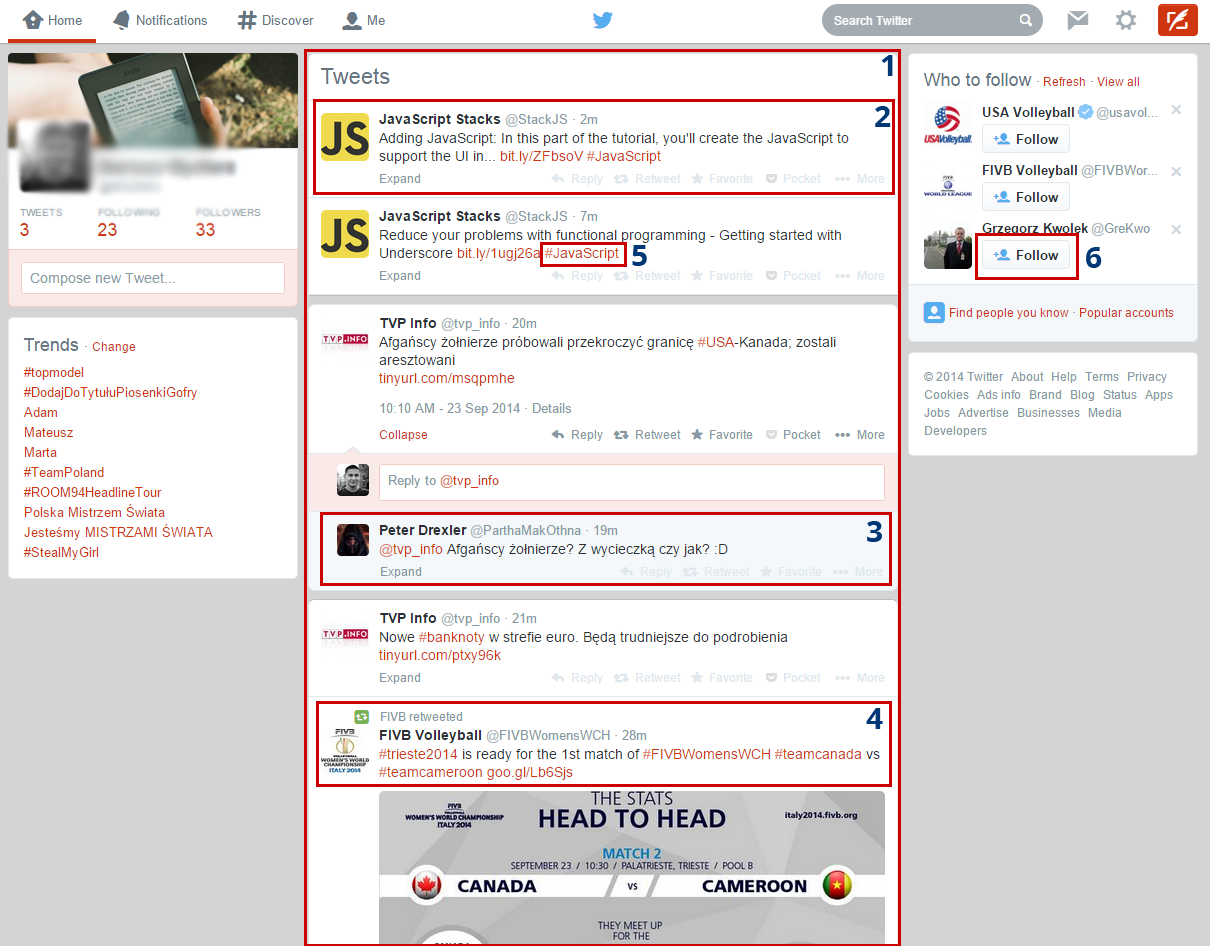
\includegraphics[width=160mm]{img/twitter-screen2.png}
\caption{Budowa serwisu Twitter}
\label{image:twitter-screen}
\end{figure}

\begin{enumerate}
  \item Ściana wpisów (ang. \textit{newsfeed}) -- inaczej strona główna 
  użytkownika, na której widzi wszystkie tweety wysłane przez osoby, które śledzi.
  
  \item Wpis (ang. \textit{tweet}) -- pojedynczy wpis/post na Twitterze; 
  maksymalna długość to 140 znaków; może dodatkowo zawierać zdjęcie lub 
  informację o geolokalizacji.

  \item Odpowiedź (ang. \textit{reply}) -- odpisanie na jakąś wiadomość w serwisie
  Twitter, skomentowanie jej; serwis łączy takie wpisy w jedną grupę, wyświetlając
  je jeden obok drugiego.
  
  \item Podanie wpisu dalej (ang. \textit{retweet}) -- oznacza przekazanie 
  jakiegoś wpisu dalej; jeśli użytkownik A użyje funkcji
  retweet dla dowolnego wpisu w serwisie, wówczas osoby śledzące użytkownika A, 
  również zobaczą ten wpis na swojej stronie głównej.
  
  \item Wyraz z symbolem kratki (ang. \textit{hashtag}) -- użycie symbolu \# 
  wraz z jakimś słowem; ułatwia rozmowy na wspólne tematy, wśród większych grup
  użytkowników (np. \textit{\#worldcupfinal} dla osób komentujących finał 
  mistrzostw świata).

  \item Śledzenie (ang. \textit{follow}) -- osób, organizacji; śledzenie 
  jakiegoś użytkownika oznacza wyświetlanie wszystkich jego wpisów na swojej 
  stronie głównej.
\end{enumerate} 

\subsection{Twitter jako źródło danych}
Twitter używany jest przez 271 milionów użytkowników wysyłających 500 
milionów wpisów dziennie\footnote{www.about.twitter.com/company}.
Szybkość komunikacji i łatwość publikacji wpisów
sprawia, że staje się medium komunikacyjnym dla wielu grup ludzi.
Odgrywał ważną rolę w wydarzeniach społeczno-politycznych,
takich jak Arabska Wiosna w 2010, czy okupowanie Wall Street w 2012 
\cite{TwitterDataAnalytics2013}.
Serwis ten jest również bardzo często wykorzystywany do komentowania wydarzeń
sportowych. W trakcie mundialu w Brazylii użytkownicy wysłali 672 miliony
wpisów z tagiem \#WorldCup \cite{TwitterStatsWorldCup}.

Popularność Twittera jako źródła informacji doprowadziła do rozwoju badań
w różnych dziedzinach. Pomoc humanitarna i w przypadku klęsk żywiołowych
jest jedną z domen, gdzie informacje z Twittera są używane w celu zapewnienia
odpowiedniej pomocy. Naukowcy wykorzystują go by przewidzieć występowanie trzęsień
ziemi i określić odpowiednich użytkowników, których śledzenie dostarcza informacji
związanych z katastrofą \cite{TwitterDataAnalytics2013}.

\subsubsection{Sposób dostępu do danych}
Dostęp do danych z Twittera możemy uzyskać na dwa sposoby.
Pierwszy to Streaming API\footnote{www.dev.twitter.com/streaming/overview}.
Aby z niego korzystać należy napisać program, który nasłuchuje pojawiających się
na żywo wpisów. Co ważne ich liczba jest ograniczona do maksymalnie 1\% wszystkich
wpisów na Twitterze. Streaming API pozwala na zbieranie danych przy użyciu słów
kluczowych, określenia języka wpisów, lokalizacji i tym podobnych.

Drugim sposobem zbierania danych z Twittera jest REST 
API\footnote{www.dev.twitter.com/rest/public}. Służy ono do wykonywania
zapytań RESTowych, za pomocą których możliwe jest pobranie listy wpisów
danego użytkownika, listy jego znajomych, listy wpisów z zadanymi słowami
kluczowymi i tym podobne. W przeciwieństwie do poprzedniej metody REST API nie nasłuchuje
wpisów na żywo, a jedynie zwraca dane dostępne w momencie wysłania żądania.
Zapytania do API można wykonywać w 15 minutowych oknach, w których możliwe
jest wysłanie maksymalnie 180 zapytań, w wyniku których można uzyskać
nie więcej niż 100 wpisów (to daje nam maksymalnie 7200 wpisów na godzinę).
Co więcej wyszukiwanie wpisów przez REST API przy użyciu 
słów kluczowych w rezultacie zwraca jedynie wyniki z ostatnich
6-9 dni. 
%The Search API is not complete index of all Tweets, but instead an index of 
%recent Tweets. At the moment that index includes between 6-9 days of Tweets. 
To API bardziej przydaje się więc do tworzenia aplikacji
klienckich dla Twittera niż do zbierania danych (konsumowania ich na żywo),
gdzie lepszym rozwiązaniem jest Streaming API.



\begin{comment}
Dane z Twittera można uzyskać poprzez API udostępniające 1\% wpisów.
Pozyskanie większej ich liczby wiąże się z dodatkowymi opłatami, z których
korzystają największe przedsiębiorstwa badające społeczność Twittera.
Korzystając ze Streaming API mamy możliwość konsumowania na żywo
wpisów spełniających podane kryteria wyszukiwania (np. słowa kluczowe, lokalizację).
Serwis udostępnia również REST API, które służy do pozyskiwania statycznych danych
-- wpisów użytkownika w momencie wysłania żądania, listy jego obserwowanych,
czy szczegółowych danych go dotyczących. Tweety zawierające dane o lokalizacji
są do klienta przesyłane wraz z tą informacją, dzięki czemu możliwe jest
skorzystanie z nich w analizach.


Co ciekawe zaledwie około 2\% wpisów posiada informację o lokalizacji wysłania
ustaloną na podstawie współrzędnych dostarczonych przez system 
GPS\cite{GnipGeotaggedNumber}.
\end{comment}